%
% File: chap02.tex
%
\let\textcircled=\pgftextcircled
\chapter{Results}
\label{chap:result}

\initial{I}n this section, the results are given. And they're shit. This presents what results are shown, etc. Not much to say actually, besides showing the plot. THis is a simple lab. We discuss about the uncertainties too.

\section{Results}

Figure~\ref{fig:flux2} illustrates the position of each sample versus the calculated flux in that area. From the figure, we may surmise that the samples were not fully centered, as we would expect a symmetrical curve centered around the zero position. Instead, we see a skewing to the left (corresponding to down in the reactor), meaning that flux was greatest in the lower areas, and peaked around the $-58\ \text{mm}$ position.

\begin{figure}[t!]
	\centering
	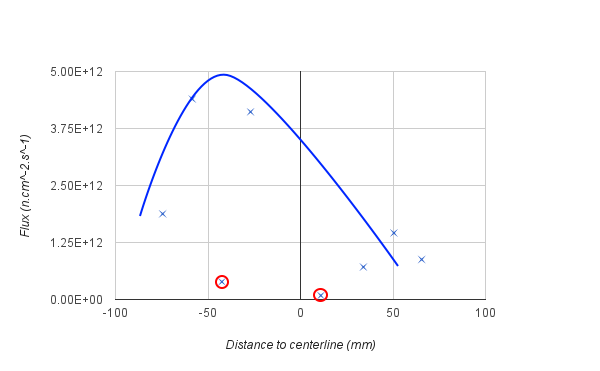
\includegraphics[height=0.4\textheight]{fig02/flux2.png}
	\mycaption[Thermal neutron flux seen in the samples]{Thermal neutron flux seen in the samples.}
	\label{fig:flux2}
\end{figure}

We see in the above graph two obviously erroneous points, which we have circled in red. These points have been disregarded and will be further examined in the errors and uncertainty portion of the report delineated below. It is possible that with more accurate measurements and sample points, we would see a peak nearer the zero position, meaning that flux is maximized at this point. 

From our usable data, a maximum value of $0.296\ \micro\text{Ci}$ was achieved at the $-27\ \text{mm}$ position. From our measured mass of $0.42\ \text{mg}$, this activity corresponded to a neutron flux of $4.11 * 10^{12}\ n.cm^{-2}.s^{-1}$. A maximum flux of $4.40 * 10^{12}\ n.cm^{-2}.s^{-1}$ was found at position $-58\ \text{mm}$. This flux is a decade off from the expected maximum flux of $1$ to $3 * 10^{13}\ n.cm^{-2}.s^{-1}$.

A full presentation of sample positions, masses, activity, and flux values are presented in the appendix.

\section{Uncertainties}

Several errors persist through this lab that caused a variance in our expected results. 

First, we used a very small amount of mass in our samples. This lends itself to several errors. With this small amount of salt in the container, even small variance in the scale’s reading can lead to huge deviations from our expected values. Small currents of air could have affected our measurements on the scale, even though the scale area has a small box in order to prevent such an event. When we use ~0.4 mg of salt, every single grain is important. Most containers needed only 2 or 3 grains of salt to meet our weight requirement. This means that salt sticking to the outside of our container could have skewed our weight measurements. When this salt was brushed or washed off the outside of the container, our assumed weight would no longer be valid, and our calculations would be tremendously off. 

Irradiation times also play a small role in our uncertainty calculations. Our sample was irradiated for a five minute fetch of time, however our calculations had assumed a ten minute irradiation period. This, initially, lead to a large deviation of observed values of activity from our expected values. 

A human error may have been introduced during irradiation. It is possible that some of the sample containers were not entirely shut. This would lead to water penetrating the container, and washing away the salt. 

During extraction and activity measurement of the samples, several human errors may have been introduced to cause a large deviation from our expected results. During the extraction of the sample containers from the tube, tweezers were used to pull containers from a Styrofoam housing. Due to the orientation of the plastic containers in the Styrofoam, it was very difficult to extract the container with the tweezers without popping the pressure-sensitive lid open. Lid-opening occurred on several occasions, though we were careful to try to not spill any salt, it is possible that a grain or two fell out of the containers, which may explain the variance in our results. It is recommended that if the experiment is repeated, that the containers be oriented differently in the styrofoam housing. 

When the activity of the salt was measured, it was placed on the gamma spectrometer in the plastic container. It is possible that some of the salt stuck to the top side of the plastic container instead of sitting at the bottom, immediately on top of the detector. This could cause small deviations and incongruities in the activity measurements of the samples. 
